% This is LLNCS.DEM the demonstration file of
% the LaTeX macro package from Springer-Verlag
% for Lecture Notes in Computer Science,
% version 2.4 for LaTeX2e as of 16. April 2010
%
\documentclass{llncs}
%
\usepackage{makeidx}  % allows for indexgeneration
\usepackage[table]{xcolor}
\usepackage{graphicx}
	\graphicspath{{images/}} 
\usepackage{cite}
\usepackage{courier}
\usepackage{hyperref}
    \hypersetup{colorlinks=true,allcolors=blue}
\usepackage{listings}
	\lstset{
  		basicstyle=\ttfamily,
  		frame=none,
  		breaklines=true,
  		numbers=left,
  		xleftmargin=2em,
  		framexleftmargin=0em,
    	emphstyle=\textbf,
    	float=t
	}
	\lstdefinestyle{ocl}{
  		emph={
        	context, inv
    	}
	}
	\lstdefinestyle{cbp}{
  		emph={
        	session, create, of, type,
        	set, to, add, hire
    	}
	}
	\lstdefinestyle{xmi}{
  		emph={
        	Employee, manages
    	}
	}

\begin{document}
\renewcommand{\thelstlisting}{\arabic{lstlisting}}
\renewcommand{\labelitemi}{$\bullet$}

\title{Turning Models Inside Out}
%
\titlerunning{Turning Models Inside Out}  % abbreviated title (for running head)
%                                     also used for the TOC unless
%                                     \toctitle is used
%
\author{Dimitris Kolovos \and Fiona Polack \and Alfa Yohannis}
%
\authorrunning{Ivar Ekeland et al.} % abbreviated author list (for running head)
%
%%%% list of authors for the TOC (use if author list has to be modified)
%\tocauthor{Ivar Ekeland, Roger Temam, Jeffrey Dean, David Grove,
%Craig Chambers, Kim B. Bruce, and Elisa Bertino}
%
\institute{Department of Computer Science, University of York, United Kingdom\\
\email{\{dimitris.kolovos, fiona.polack, ary506\}@york.ac.uk}}

\maketitle              % typeset the title of the contribution

\begin{abstract}
To reap the benefits of Model-Based Software Engineering in the context of large and complex systems, the ability to process large models in an incremental fashion as they evolve is essential. ``Incremental" means that the amount of time it takes to execute a model processing operation on a modified model should be proportional to the size of the change, as opposed to the size of the entire model. Current incremental model processing techniques either only deliver marginal performance benefits due to slow and imprecise model change detection capabilities or are limited to a single-developer environment---which is not realistic for real-world software development projects. The aim of this research is to enable high-performance incremental model processing. Instead of persisting snapshots of the state of models, we propose turning models inside out and persisting their change history. The proposed approach has the potential to deliver step-change performance benefits in incremental model processing, which will enable a wide range of advantages and novel capabilities.
\end{abstract}

\section{Introduction}
\label{Introduction}
Model-Based Software Engineering (MBSE) is a software engineering approach that promotes models to first-class artefacts of the software development and maintenance lifecycle. In MBSE, rigorously defined---and often domain-specific---models are used to capture the essence of (parts of) the system under development at an appropriate level of abstraction, and are then used to reason about properties of the system (e.g. via model checking and simulation), and eventually to produce low-level implementation artefacts (e.g. source code, configuration scripts) in an automated fashion. MBSE has demonstrated a strong potential to drastically improve productivity and consistency in software development by reducing development time \cite{jaaksi2002developing}, cost \cite{davies2014model}, and the probability of human-induced errors \cite{mohagheghi2013empirical}. This is widely recognised in industry where studies (e.g. \cite{liebel2014assessing, hutchinson2011empirical}) have shown that model-based development is used extensively.

This paper is structured as follows. Section \ref{The Key-Challenge of Incrementality} reviews the key-challenge of incrementality of change-based model. Section \ref{Identifying Changes in Models} briefly presents two existing approaches for identifying changes in models. Section \ref{Proposed Approach} overviews our proposed approach. The potential benefits and novel capabilities, as well as the challenges of change-based model are presented in Sect. \ref{Benefits and Novel Capabilities} and Sect. \ref{Challenges} respectively. Section \ref{Evaluation Strategy} presents our evaluation strategy. Section \ref{Conclusions} concludes this paper.

\section{The Key-Challenge of Incrementality}
\label{The Key-Challenge of Incrementality}
As MBSE is used for the development of larger and more complex systems in a variety of domains, the ability to process (e.g. validate, transform, generate code from) large models in an incremental fashion as they evolve becomes essential. ``Incremental'' in this context means that the amount of time it takes to update the results of a model processing operation on a modified model, is generally proportional to the size of the change, as opposed to the size of the model. To illustrate the concept of incrementality, a contrived running example is used where, after every modification to an organisational chart model (see Fig. \ref{image1}), the model needs to be:

\begin{itemize}
\item Validated against a domain-specific constraint (that no employee directly manages more than 7 other employees).
\item Transformed into a number of employee reports (plain text files, one for each employee) through a model-to-text transformation. Each report should contain the name of the employee, and the names of her direct subordinates.
\end{itemize}

Figures \ref{image1} and \ref{image2} are two consecutive versions of a sample organisational chart model. When the validation constraint is evaluated against the first version of the model (Fig. \ref{image1}), it verifies that all three employees manage fewer than 7 other employees, and the model-to-text transformation then produces three text files that correspond to the employees in the model.

\begin{figure}[b!]
\centering
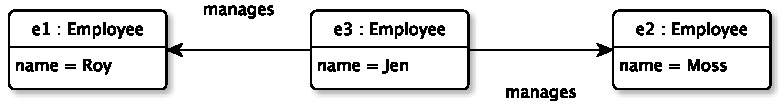
\includegraphics[width=\linewidth]{image1}
\caption{Initial version of the organisational chart model.}
\label{image1}
\end{figure}

\begin{figure}[b!]
\centering
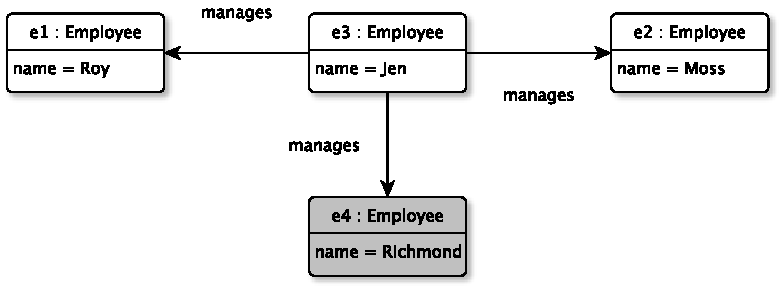
\includegraphics[width=\linewidth]{image2}
\caption{Modified version of the organisational chart model of Fig. \ref{image1}.}
\label{image2}
\end{figure}

In the sequel, in Fig. \ref{image2}, the model is updated to reflect that a new employee has been hired (Richmond) under the management of Jen. 

A non-incremental model validation engine, would treat the model of Fig. \ref{image2} as if it was a new model and would evaluate the constraint above against every employee in the model. An incremental model validation engine on the other hand would identify that the previously established satisfaction of the constraint for employees Moss and Roy cannot have been possibly compromised by the changes made, and would only re-evaluate the constraint for Jen and Richmond instead. 

Similarly, a non-incremental model-to-text transformation, would generate all employee reports from scratch (overwriting any previous versions of them\footnote{Most code generation engines support preservation of hand-written content in existing files through ``protected regions" mechanisms, however this is not important for the purpose of this discussion}). On the contrary, an incremental model-to-text transformation, would identify that it only needs to generate a new report for the new employee (Richmond), and to recompute and overwrite the contents of Jen's report (as she is now managing an additional employee)---but not the reports of Moss or Roy, as these cannot have been affected by the changes made to the model.

While the overhead of executing transformations and validation constraints on small models like the one in Fig. \ref{image2} is negligible, non-incremental execution can become a significant bottleneck for large evolving models. As stressed in Selic’s seminal work \cite{selic2003pragmatics}, with reference to model-to-text transformation, ``... \emph{this is particularly true in the latter phases of the development cycle, when programmers make many small changes as they fine-tune the system. To keep this overhead low, it is crucial for the code generators to have sophisticated change impact analysis capabilities that minimize the amount of code regeneration}".

As demonstrated by the pioneering work of Egyed \cite{egyed2011automatically}, to achieve incremental re-execution of (deterministic) queries on structured models, an execution engine needs to:

\begin{enumerate}
\item Record model element property accesses during the initial execution of the queries;
\item Identify new and deleted elements, and modified model element properties in the new version
of the model;
\item Combine the information collected in the steps above to identify the subset of (potentially) affected queries that need to be re-executed.
\end{enumerate}

To briefly illustrate Egyed’s approach, we use an OCL\footnote{The Object Constraint Language is a constraint language standardised by the Object Management Group (OMG).} implementation of the domain-specific constraint in List. \ref{constraint}.


\begin{lstlisting}[style=ocl,caption={OCL constraint requiring that no employee directly manages more than 7 other employees.},label=constraint]
context Employee
inv NoMoreThan7: self.manages->size() <= 7
\end{lstlisting}

During the initial evaluation of the constraint on the model of Fig. \ref{image1}, an incremental OCL engine would compute the property access trace displayed in Table \ref{table1} as a side-product. Now, when the model is updated (Fig. \ref{image2}), the execution engine can identify that:

\begin{itemize}
\item There is new element in the model (\emph{e4} - Richmond) for which the constraint has not been evaluated;
\item The value of the manages property of Jen (\emph{e3}) has changed and as such it needs to re-evaluate
the constraint on this model-element.
\end{itemize}

\begin{table}[h!]
\centering
\caption{Property-access trace of the evaluation of the constraint in List. \ref{constraint} on the model of Fig. \ref{image1}.}
\begin{tabular}{p{4.8cm} p{2.1cm} p{2cm} p{2.1cm}}
\hline 
\rule[-1ex]{0pt}{2.5ex}\textbf{Constraint} & \textbf{Context} & \textbf{Accessed Element} & \textbf{Accessed Property} \\ 
\hline 
\emph{Employee.NoMoreThan7}  & \emph{e1} & \emph{e1} & \emph{manages} \\ 
\emph{Employee.NoMoreThan7}  & \emph{e2} & \emph{e2} & \emph{manages} \\ 
\emph{Employee.NoMoreThan7}  & \emph{e3} & \emph{e3} & \emph{manages} \\ 
\hline 
\end{tabular} 
\label{table1}
\end{table}

Egyed has shown that the property-access recording approach is applicable to queries of arbitrary complexity, as long as they are deterministic. Moreover, work derived from Egyed’s approach has shown that variants of this approach can be used to achieve incrementality in a wide range of model processing operations, including model-to-model transformation \cite{jouault2010towards}, model-to-text transformation \cite{ogunyomi2015property}, model validation, and pattern matching \cite{rath2012derived}---as long as changes to models can be precisely identified (step 2 in the list above).

\section{Identifying Changes in Models}
\label{Identifying Changes in Models}
There are two approaches in the literature for identifying changes in models in order to enable incremental re-execution of model processing operations.

\textbf{Notifications}. In this approach, the incremental execution engine needs to hook into the notification facilities provided by the modelling tool through which the developer edits the model, so that the engine can directly receive notifications as soon as changes happen (e.g. a new employee (\emph{e4}) has been added, the name property of employee \emph{e4} has been changed to ``Richmond"). This is an approach taken by the IncQuery incremental pattern matching framework \cite{rath2012derived} and the ReactiveATL incremental model-to-model transformation engine \cite{ogunyomi2015property}. The main advantage of this approach is that precise and fine-grained change notifications are provided for free by the modelling tool (and thus do not need to be computed by the execution engine---which as discussed below can be expensive and inefficient). On the downside, this approach is a poor fit for collaborative development settings
where modelling and automated model processing activities are performed by different members of the team (e.g. in a setup where several engineers can edit and validate a model, but only one of them is responsible for regenerating the source code when the model reaches a desirable degree of maturity).

\textbf{Model Differencing}. This approach eliminates the coupling between modelling tools and incremental execution engines. Instead of depending on live notifications, in this approach the developer in charge of automated model processing, needs to maintain a copy of the last version of the model that the model processing program (e.g. the model-to-text transformation) was executed upon, so that it can be compared against the current version of the model (e.g. using a model-differencing framework such as SiDiff or EMFCompare) and the delta can be computed on demand. The main advantage of this approach is that it works well in a collaborative development environment where---typically---developers have distinct roles and responsibilities. On the downside, model comparison and differencing are computationally expensive and memory-greedy (both versions of the model need to be loaded into memory before they can be compared), thus largely undermining the time and resource saving potentials of incremental re-execution. This approach is adopted by the Xpand model-to-text transformation language. According to the developers of the language, using this approach, a speed-up of only around 50\% is observed compared to non-incremental transformation\footnote{\url{http://wiki.eclipse.org/Xpand/New_And_Noteworthy\#Incremental_Generation}}, which is consistent with our experience from using Xpand.

In summary, incremental model processing currently delivers significant performance benefits only
in a single-developer environment where the modeller is also responsible for performing all the (incremental) model processing operations. As a result, in collaborative development environments,
\textbf{developers need to either forgo incremental model processing altogether, or to work around
this limitation by manually steering model processing programs to process only subsets of
their models, which is cumbersome and error prone}.

\section{Proposed Approach}
\label{Proposed Approach}
The ambition of this research is to enable high-performance incremental model management in collaborative software development environments by \textbf{challenging one of the fundamental assumptions} of contemporary modelling frameworks and tools: As opposed to persisting snapshots of the state of models (which is what virtually all modelling tools and frameworks currently do), we propose \textbf{turning models inside out} and \textbf{persisting their change history instead}.

To illustrate the proposed approach, List. \ref{xmimodel} shows a state-based representation of the model of Fig. \ref{image2} in (simplified) XMI\footnote{The XML Metadata Interchange (XMI) format is a widely-used XML-based model persistence and exchange format standardised by the Object Management Group.}, and List. \ref{cbpmodel1} shows the proposed equivalent change-based representation of the same model. Instead of a snapshot of the state of the model, the representation of List. \ref{cbpmodel1} captures the complete sequence of change events (create/set/add/remove/delete) that were performed on the model since its creation, organised in editing sessions (2 editing sessions in the case of this model). Replaying these changes produces the same state as the one captured in List. \ref{xmimodel}, so the proposed representation carries at least as much information as the state-based representation.

The keen-eyed reader will observe that such a representation is particularly suitable for incremental model processing. For example, if the model-to-text transformation discussed above ``remembers" that in its previous invocation it had processed up to editing session \emph{s1} of the model, it can readily identify the changes that have been made to the model since then (i.e. in session \emph{s2} –- lines 11-13) instead of having to rediscover them through (expensive) state-based model differencing.

\begin{lstlisting}[style=xmi,caption={State-based representation of the model of Figure \ref{image2} in (simplified) XMI.},label=xmimodel]
<Employee xmi:id="e2" name="Jen">
    <manages xmi:id="e1" name="Roy"/>
    <manages xmi:id="e3" name="Moss"/>
    <manages xmi:id="e4" name="Richmond"/>
</Employee>
\end{lstlisting}

\begin{lstlisting}[style=cbp,caption={Proposed change-based representation of the model of Figure \ref{image2}.},label=cbpmodel1]
session s1
create e1 of type Employee
set name of e1 to "Roy"
create e2 of type Employee
set name of e2 to "Moss"
create e3 of type Employee
set name of e3 to "Jen"
add e1 to manages of e3
add e2 to manages of e3
session s2
create e4 of type Employee
set name of e4 to "Richmond"
add e4 to manages of e3
\end{lstlisting}

\section{Benefits and Novel Capabilities}
\label{Benefits and Novel Capabilities}
Beyond facilitating incremental processing, the proposed representation also has the potential to deliver a wide range of benefits and novel capabilities, compared to the currently prevalent state-based representations, some of which are discussed below.

\begin{itemize}
\item With appropriate tool support, modellers will be able to ``replay" (part of) the change history of a model (e.g. to understand design decisions made by other developers, for training purposes). In state-based approaches, this can be partly achieved if models are stored in a version-control repository (e.g. Git), however the granularity would only be at the commit level.
\item By analysing models serialised in the proposed representation, modelling language and tool vendors will be able to develop deeper insights about how modellers actually use these languages/tools in practice, and utilise this information to guide the evolution of the language/tool.
\item By attaching additional information to each session (e.g. the id of the developer, references to external documents/URLs), sequences of changes can be traced back to the developer that made them, or to requirements/bug reports that triggered them.
\item Persisting changes to large models after an editing session will be significantly faster compared to serialising the entire state of the model, as only changes made during the session will need to be appended to the model file.
\item As an extension of this approach, domain-specific change-based serialisation formats can be developed, which will be able to capture semantically-rich composite domain-specific changes in addition to primitive change operations. For example, List. \ref{cbpmodel2} makes use of a domain-specific hire change which adds a new employee to the model and sets their name, as an atomic action.
\item The performance and precision of model comparison and merging can be substantially improved, particularly for large models with shared editing histories.
\end{itemize}

\begin{lstlisting}[style=cbp,caption={Language-specific change-based representation of the model of Figure \ref{image1}.},label=cbpmodel2]
session s1
hire e1 "Roy"
hire e2 "Moss"
hire e3 "Jen"
add e1 to manages of e3
add e2 to manages of e3
session s2
hire e3 "Richmond"
add e4 to manages of e3
\end{lstlisting}

\section{Challenges}
\label{Challenges}
The proposed approach also comes with a number of challenges that this research will need to overcome.

\textbf{Loading Overhead}. While, as discussed above, persisting changes to large models is expected to be much faster and resource-efficient compared to state-based approaches, loading models into memory by naively replaying the entire change history is expected to have a significant overhead. To address this challenge:

\begin{itemize}
\item We will develop dedicated algorithms and data structures that will reduce the cost of change-based model loading. For example, for single-value model element attributes (e.g. \emph{Employee::name} in the example above) only the last value change can be replayed at the model level. Other types of changes (e.g. additions/removals of elements in multi-valued containment/opposite references) are not as straightforward and require substantial research to handle efficiently.
\end{itemize}

\textbf{Fast-Growing Model Files}. Persisting models in a change-based format means that model files will keep growing in size during their evolution significantly faster than their state-based counterparts. For example, while deleting a model element in a state-based representation is likely to lead to a
smaller model file, the same action in a change-based format is guaranteed to increase the size of the model file (as the deletion needs to be recorded on top of all the previous changes). To address this challenge:

\begin{itemize}
\item We will propose sound change-compression operations that developers will be able to invoke on demand to reduce the size of a model, by sacrificing some information (e.g. compress changes made in the context of older editing sessions) in a controlled way;
\item We will develop a compact textual format that will minimise the amount of space required to record a change (a textual line-separated format is desirable to maintain compatibility with file-based version control systems);
\item We will propose a hybrid model persistence format which will be able to incorporate both change-based and state-based information. 
\end{itemize}

\textbf{Tool Support}. For the proposed approach to have a strong practical impact, it needs to be supported by modelling, model processing (e.g. transformation) languages, and model management (e.g. comparison, differencing, merging) tools. To address this challenge:

\begin{itemize}
\item We will extend existing open-source graphical editor frameworks such as Sirius\footnote{\url{http://eclipse.org/sirius/}}, GMF\footnote{\url{http://www.eclipse.org/gmf-tooling/}}, and Papyrus\footnote{\url{http://eclipse.org/papyrus/}} so that they can support the development of editors that persist models in the proposed change-based format.
\item We will extend open-source model processing languages so that they can incrementally process change-based models. We will initially target languages of the well-established Epsilon family, which the PI is leading, but we will explore how other languages that already support incremental execution (e.g. OCL, ATL, IncQuery) can be extended with similar capabilities.
\item We will devise dedicated model comparison, differencing and merging algorithms, to support collaborative development using change-based models.
\end{itemize}

\section{Evaluation Strategy}
\label{Evaluation Strategy}
The findings of the research will be evaluated in the small in the context of the tasks in which they will be developed, and in the large through industrial case studies.

For the first type of evaluation (in the small), where there are existing approaches that the algorithms and tools developed in this research seek to outperform (e.g. change-based incremental validation vs. state-based incremental validation), comparative evaluation will be conducted to assess the benefits and limitations of our approaches. For algorithms and tools that have no direct competitors in the literature, their contributions will be assessed in comparison to the baseline they seek to improve (e.g. in this case, persisting full change histories).

Evaluation in the large will be conducted through appropriate case studies in collaboration with industrial peers---modelling tool vendors (e.g. Modelio UML) and heavy adopters of automated model processing (e.g. Rolls-Royce, Thales, Atos, and Siemens).

\section{Conclusions}
\label{Conclusions}
Through turning models inside out and persisting their change history, this paper propose change-based model as an approach to enable high-performance incremental model processing in collaborative development settings. The proposed approach has the potential to deliver step-change performance benefits (e.g. faster model persistence, comparison, and merging) in incremental model processing, which has the potential to enable analytics of models (e.g. trace and replay model history, develop insight how modelling tools used). For future works, we will develop dedicated algorithms and data structures to reduce the cost of change-based model loading, a change-based format to persist models, change-compression operations to reduce the size of a model, a compact textual format to minimise space size, a hybrid model persistence format to incorporate change-based and state-based models, and support for existing modelling tools. Comparative evaluation will be conducted to assess the benefits and limitation of our approaches by comparing them to existing algorithms, tools, or baselines that they seek to improve.

\subsubsection*{Acknowledgments.} This work is part of a doctoral scholarship managed by \emph{Lembaga Pengelola Dana Pendidikan Indonesia} (Indonesia Endowment Fund for Education).

\bibliography{references} 
\bibliographystyle{splncs}

\end{document}
